\documentclass[11pt,oneside]{uhthesis}
%\documentclass[11pt,oneside]{report}
\usepackage{subfigure}
\usepackage[linesnumbered,lined,titlenumbered,ruled]{algorithm2e}
\usepackage{amsmath}
\usepackage{amssymb}
\usepackage{amsbsy}
\usepackage{mathpazo}
\usepackage{float}
\usepackage{braket}
\setlength {\marginparwidth }{3cm}
\usepackage{todonotes}

\usepackage[spanish]{babel}
\usepackage{graphicx}

\usepackage{listings}
\usepackage{color}
\usepackage{booktabs}
\usepackage{multirow}
\usepackage{ragged2e}

\floatstyle{ruled}
\restylefloat{table}
\usepackage{listings}
\usepackage{color}

\definecolor{dkgreen}{rgb}{0,0.6,0}
\definecolor{gray}{rgb}{0.2,0,0}
\definecolor{mauve}{rgb}{0.58,0,0.82}

\lstset{language=Lisp,
	aboveskip=10mm,
	belowskip=10mm,
	showstringspaces=false,
	columns=flexible,
	basicstyle={\small\ttfamily},
	keywordstyle=\color{blue},
	commentstyle=\color{dkgreen},
	stringstyle=\color{mauve},
	breaklines=true,
	breakatwhitespace=true,
	tabsize=3,
	numbers=left, numberstyle=\tiny, stepnumber=1,firstnumber=1,
	numbersep=5pt
}

\renewcommand{\tablename}{Tabla}
\title{Sistema para la integración de herramientas para la solución ágil de Problemas de Enrutamiento de Vehículos}
\author{Rodrigo García Gómez}
\advisor{MSc. Fernando Rodríguez Flores}
\coadvisor{}
\degree{Licenciado en Ciencias de la Computación}
\faculty{Facultad de Matemática y Computación}
\date{Noviembre de 2022}
\logo{Graphics/uhlogo}

\renewcommand{\vec}[1]{\boldsymbol{#1}}
\newcommand{\diff}[1]{\ensuremath{\mathrm{d}#1}}

\begin{document}
\selectlanguage{spanish}

%\frontmatter
\maketitle

\begin{dedication}
	\textit{
		A mis amigos\\
		A mi familia\\
		A Juan\\
		A mi Mamá.}
\end{dedication}
\chapter*{Agradecimientos}\label{chapter:agradecimientos}

Un agradecimiento a Héctor Masson Rosquete, Jose Jorge Rodríguez, Heidy Abreu Fumero y Camila Pérez Mosquera. La combinación de sus ideas hizo posible esta tesis.\\

A mi tutor Fernando Rodríguez por su guía, paciencia y atención.\\

A Juan y mi madre por dedicar gran parte de sus vidas a eliminar los problemas de la mía.\\


% Fernado




\begin{opinion}	
	
En los últimos años en nuestra facultad se han desarrollado varias tesis de licenciatura que tributan a agilizar el proceso de solución de un VRP, y aunque cada una de ellas han resuelto una arista del problema no era posible usarlas para resolver problemas, porque cada una existía independientemente de las demás.  Gracias al trabajo de Rodrigo, es posible usar los resultados de todas esas tesis en un único producto.

Uno de los méritos del trabajo es que Rodrigo tuvo que leer, entender y modificar más de 10 000 líneas de código en un lenguaje completamente distinto a todo lo conocido por él hasta ese momento.  Eso lo hizo de una manera excelente, al punto de poder discutir con los autores (de tú a tú) sobre cualquier aspecto del código.

A mi juicio, esto demuestra que Rodrigo es capaz de utilizar los conocimientos adquiridos durante la carrera de una manera creativa, puede identificar y solucionar problemas que aparezcan durante la investigación y ciertamente puede adquirir de manera autodidacta los conocimientos y habilidades que necesite.

Por todo lo anterior creo que estamos en presencia de un excelente científico de la computación, que al igual que el trabajo, merece la máxima calificación.


\vspace{1cm}


\begin{flushright}
	\underline{\hspace{6.5cm}}\\
	MSc. Fernando Raúl Rodríguez Flores
	
	Facultad de Matemática y Computación
	
	Universidad de la Habana
	
	Noviembre, 2022
\end{flushright}

\end{opinion}
\begin{abstract}
En este trabajo se propone un sistema capaz de resolver variantes de VRP con metaheurísticas de búsqueda local, permitiendo reducir el tiempo de solución a un par de días. Para lograrlo se combinan tres herramientas. La primera permite evaluar soluciones vecinas de forma eficiente y automática mediante un Grafo de Evaluación, la segunda permite explorar vecindades a partir de cualquier estrategia mediante un Árbol de vecindad y la tercera permite generar funciones de exploración que combinan cualesquiera estrategias de exploración y selección. Estas herramientas fueron desarrolladas en tres tesis de licenciatura diferentes pero quedaron como marcos teóricos que no podían funcionar por sí solos. En este trabajo se combinó estas herramientas en un sistema completo y funcional.

\end{abstract}

\begin{enabstract}
In this work, a system capable of solving VRP variants with local search metaheuristics is proposed, reducing the solution time to a couple of days. To achieve this, three tools are combined. The first allows to evaluate neighbor solutions efficiently and automatically using of an Evaluation Graph, the second allows to explore neighborhoods from any strategy using a Neighborhood Tree and the third allows to generate exploration functions that combine any exploration and selection strategy. These tools were developed in three different thesis but remained as teorical works that could not be used by their own. In this work, these tools were combined in a complete and functional system.	
\end{enabstract}
\tableofcontents
\listoffigures


%\mainmatter
	
%===================================================================================
% Chapter: Introduction
%===================================================================================
\chapter*{Introducción}\label{chapter:introduction}
\addcontentsline{toc}{chapter}{Introducción}
%===================================================================================

\qquad 
Los costos por transportación pueden representar más de la mitad de los costos logísticos de una empresa \cite{factoid}. Esto implica que para empresas con capitales millonarios, una buena planeación de sus rutas de transportación puede representar un ahorro igualmente millonario.

El problema de enrutamiento de vehículos (VRP por sus siglas en inglés) es un problema de optimización combinatoria cuyo objetivo en su forma más simple es, dado un conjunto de clientes, un depósito y una flota de vehículos, encontrar una asignación de rutas que optimice ciertos criterios tales como tiempo y costos de transportación.

En la literatura se reportan múltiples variantes para este problema como el Problema de Enrutamiento de Vehículos con restricciones de capacidad (CVRP) \cite{CVRP}, el Problema de Enrutamiento de Vehículos con ventanas de tiempo \cite{VRPTW} y el Problema de Enrutamiento de Vehículos con recogida y entrega (VRPPD) \cite{2002vehicle}, por citar sólo algunas de las más estudiadas. Cada variante tiene restricciones propias, por lo que resulta difícil la creación de un método de solución universal para cualquier VRP.

Estos problemas son NP-duros, esto implica que no existen soluciones exactas para conjuntos de datos reales y por tanto, se utilizan técnicas aproximadas como heurísticas y metaheurísticas que han sido objeto de estudio por décadas \cite{1964scheduling,1974networks,1981complexity,1997tabu,2002vehicle}.

En particular, los algoritmos de búsqueda local han mostrado buenos resultados en los últimos tiempos \cite{ALNS-2007,Osman-1996,Vns-Component-2013}.

El proceso de solución de un Problema de Enrutamiento de Vehículos específico es complejo y su solución puede tomar tiempo. Por ejemplo, hasta un año en caso de una maestría \cite{Alina2010} y varios años en caso de una tesis de doctorado \cite{Alina2017}.

Desde hace varios años, comenzando por \cite{Camila}, en la facultad de Matemática y Computación de La Universidad de La Habana se han desarrollado varias investigaciones con el objetivo de agilizar el tiempo que toma resolver una variante específica de VRP. Para ello se propone utilizar una metaheurística de búsqueda local (IVNS) que permite considerar infinitos criterios de vecindad para un problema, a partir de gramáticas libres del contexto. Luego, en \cite{Daniela} se propone una forma de obtener automáticamente, a partir de la descripción del problema, la gramática necesitada por IVNS. En \cite{JJ} se propone una manera de calcular el costo de un vecino en casi cualquier variante de VRP y para ello se utiliza un Grafo de Evaluación. En \cite{Hector} se plantean formas automáticas para explorar vecindades de distintas maneras mediante un Árbol de Vecindad. Finalmente, en \cite{Heidy} se propone una vía para combinar estrategias de exploración y selección sin tener que programar todas las combinaciones posibles a través de un generador de funciones de exploración. Cada una de estas herramientas resuelve un problema por separado, pero hasta ahora no era posible su integración. Si se lograran integrar sería posible resolver cualquier problema de VRP utilizando cualquier combinación de estrategias de exploración y criterios de vecindad a partir de \cite{Hector} y \cite{Hector}. Además usando infinitos criterios de vecindad al combinar lo propuesto en \cite{Camila} y \cite{Daniela}. La única restricción estaría en que los vecinos fueran calculables por lo propuesto en \cite{JJ}.

En este trabajo se propone una herramienta que permite integrar el Grafo de Evaluación de \cite{JJ}, con el Árbol de Vecindad de \cite{Hector} y el generador de funciones de exploración de \cite{Heidy}. Por ahora no es objetivo integrar el sistema con IVNS y por tanto se proponen otras metaheurísticas de búsqueda local como VNS \cite{Vns-Component-2013,Amous-2017}.

Con el sistema propuesto, resolver una variante de VRP se traduce en definir cómo se evalúa una única solución y definir, en un lenguaje casi natural, qué estrategias de exploración y criterios de vecindad se quieren utilizar.

\subsection*{Objetivos}
El objetivo general de este trabajo es diseñar e implementar un sistema que permita calcular los costos de cualquier vecino usando el Grafo de Evaluación de \cite{JJ}, que las vecindades se exploren usando el Árbol de Vecindad de \cite{Hector}, que las estrategias de exploración y selección se puedan combinar con lo propuesto en \cite{Heidy} y, por tanto, resolver variantes de VRP a partir únicamente del código de evaluación de una solución.

Para lograr los objetivos generales se han trazado los siguientes objetivos específicos:

\begin{enumerate}
	\item Consultar literatura especializada sobre el estado del arte de los problemas VRP.
	\item Estudiar las ideas y códigos relacionados con el Grafo de Evaluación \cite{JJ}, el Árbol de Vecindad \cite{Heidy}, y el generador de funciones de exploración \cite{Hector}.
	\item Diseñar e implementar un sistema que combine estas ideas para resolver distintas variantes de VRP a partir de la evaluación de una solución.
	\item Analizar los resultados obtenidos. Para ello se utiliza el sistema implementado para resolver, con muy poco esfuerzo humano variantes de VRP.
\end{enumerate}
El presente documento está organizado en 5 capítulos.


En el capítulo \ref{Chapter: Tools} se describen los elementos fundamentales del Problemas de Enrutamiento de Vehículos. En el capítulo \ref{Chapter: Tools} se describen las características de las tesis que se combinan en este trabajo \cite{JJ,Heidy,Hector}. El capítulo \ref{chapter:Solution} describe el sistema que se implementó. En el capítulo \ref{chapter:Tutorial} se describe el método de uso del sistema para describir y resolver variantes de VRP. En el capítulo \ref{chapter:Extension} se muestra cómo extender este sistema. En el capítulo \ref{chapter:Results} se exponen los resultados alcanzados. En el capítulo \ref{chapter:conclusions} se ofrecen las conclusiones y se brindan algunas recomendaciones para trabajos futuros.






\chapter{Problemas de Enrutamiento de Vehículos y métodos de búsqueda local}\label{chapter: VRP}

En este trabajo se propone un sistema que permite resolver de manera ágil cualquier de VRP utilizando algoritmos de búsqueda local. En este capítulo se presentan los elementos fundamentales de VRP y de las metaheurísticas de búsqueda local.

En la sección \ref{1-VRPintro} se describen los Problemas de Enrutamiento de Vehículos. En la sección \ref{1-local} se describen los algoritmos de búsqueda local. En \ref{1-Lisp} se presentan algunas características de Common lisp, lenguaje en que se implementó el sistema.

%\newpage

\section{Problema de Enrutamiento de Vehículos}\label{1-VRPintro}
La primera referencia al VRP es \cite{CVRP} y data de 1959. En este trabajo se describe una aplicación real de VRP, entrega de gasolina a varias estaciones de servicio. Para resolverlo, se propone un modelo matemático y una heurística para aproximar la solución.

La versión más sencilla recibe el nombre de CVRP (Capacitated Vehicle Routing Problem) \cite{CVRP} consta de una flota de vehículos que salen de un depósito y deben satisfacer las demandas de una serie de clientes. El objetivo es encontrar una distribución de rutas que se asignan a los vehículos de forma que se optimice determinada métrica (tiempo, combustible, costo total, etc). A partir de esta versión inicial se estudian diversas variantes que se pueden encontrar en la literatura:

\begin{itemize}
	\item VRPTW - VRP con ventanas de tiempo. Cada cliente posee un período de tiempo fijo durante el cual puede ser visitado \cite{VRPTW}.
	\item VRPPD - VRP con recogida y entrega. Los bienes deben ser entregados y recogidos en cantidades fijas \cite{VRPPD}.
	\item MDVRP - VRP con múltiples depósitos. Se cuenta con múltiples depósitos desde los que pueden salir los vehículos \cite{multi}.
	\item VRPB - VRP con backhauls. Los clientes se dividen en dos tipos \textit{A} y \textit{B}. Una solución de este problema debe cumplir con la restricción de que, en todas sus rutas, los clientes de tipo \textit{A} aparezcan antes que los clientes de tipo \textit{B} \cite{backhauls1998}.
\end{itemize}

Los Problemas de Enrutamiento de Vehículos son NP-Duros \cite{2002vehicle}, por lo que las soluciones exactas no son factibles para problemas reales. Para buscar aproximaciones a la solución se utilizan heurísticas y metaheurísticas. En la literatura se reporta \cite{puede} que las metaheurísticas de búsqueda local brindan buenos resultados en poco tiempo y por eso esta es la estrategia seleccionada para este trabajo. A continuación se describen los elementos fundamentales de los algoritmos de búsqueda local.

\section{Metaheurísticas de Búsqueda Local}\label{1-local}
Los algoritmos basados en búsqueda local parten de una solución a la que se llama solución actual y exploran un conjunto de soluciones a las que se les llama vecinos. Las soluciones vecinas se obtienen al aplicar sobre la solución actual un determinado criterio (llamado criterio de vecindad). Cada vecino se analiza y de ellos se escoge uno que puede sustituir o no a la solución actual en dependencia del algoritmo que se esté usando. 

En dependencia de factores como cuántos criterios de vecindad se tiene y cuándo sustituye o no la solución actual, se pueden obtener distintos algoritmos.

Para aplicar cualquier algoritmo de búsqueda local es necesario definir qué es una solución y esto se aborda en la siguiente sección.

\subsection{Representación de soluciones del VRP}\label{1-sol}
Una solución de un Problema de Enrutamiento de Vehículos describe qué clientes visita cada vehículo y en qué orden. Al recorrido de cada vehículo se le llama ruta. Usualmente las rutas se pueden representar por una lista de clientes y las soluciones como una lista de rutas. Por ejemplo, si se define a $P_1$ como un problema clásico (VRP en su versión más simple) que consta de 6 clientes: $[c_1, c_2, c_3, c_4, c_5, c_6]$, entonces una solución $s_1$ se puede definir como:

\begin{equation}
	s_1 = [(c_2,c_3), (c_1,c_4,c_5), (c_6)]
\end{equation}

En $s_1$ se muestra una solución con tres rutas. El vehículo perteneciente a la primera ($r_1$) ruta visita a $c_2$ y $c_3$, el vehículo de la segunda ruta ($r_2$) visita a $c_1$, $c_4$ y $c_5$ y el de la tercera ($r_3$) sólo visita a $c_6$. En todos los casos los recorridos comienzan y terminan en el depósito.

Una vez se definió una solución, es posible definir un criterio de vecindad.

\subsection{Criterios de vecindad}\label{1-criteria}
Un criterio de vecindad es una regla que permite, a partir de una solución actual, obtener nuevas soluciones. En el caso de VRP, estos criterios se pueden formar con modificaciones que se les aplica a los elementos de la solución actual. Algunos de estos criterios de vecindad \cite{Camila, Daniela} pueden ser: 

\begin{enumerate}
	\item Intercambiar dos clientes seleccionados aleatoriamente.
	\item Reubicar un cliente dentro de su ruta en la posición que minimice el costo de esa ruta.
	\item Mover aleatoriamente un cliente de una ruta a otra.
	\item Intercambiar dos vehículos seleccionados aleatoriamente.
\end{enumerate}

Los criterios de vecindad dependen también de la variante del problema sobre la que se trabaje. Por ejemplo, el criterio de \textit{Cambiar vehículos} no tiene sentido para el problema $P_1$ pues en este todos los vehículos son iguales.

Los criterios de vecindad se pueden describir en términos de operaciones elementales. Algunas de ellas son:

\begin{enumerate}
	\item Seleccionar una ruta \texttt{r}. 
	\item seleccionar un cliente \texttt{c} de una posición \texttt{p} de una ruta \texttt{r}.
	\item insertar un cliente \texttt{c} en una posición \texttt{p} de una ruta \texttt{r}.
\end{enumerate}

Las operaciones \textit{Seleccionar ruta}, \textit{seleccionar cliente} e \textit{insertar cliente} se representan en este trabajo con los símbolos \textit{r}, \textit{a} y \textit{b} respectivamente.

Se tiene como ejemplo el criterio \textit{Mover un cliente a cualquier ruta, en cualquier posición}. Este puede ser representado por las operaciones:

\begin{enumerate}
	\item Seleccionar ruta \texttt{$r_x$}.
	\item Seleccionar cliente \texttt{$c_x$} de la posición \texttt{$p_x$} de la ruta \texttt{$r_x$}.
	\item Seleccionar ruta \texttt{$r_y$}.
	\item Insertar cliente \texttt{$c_x$} en la ruta \texttt{$r_y$} en la posición \texttt{$p_y$}.
\end{enumerate}

A partir de un criterio de vecindad y una solución inicial se pueden generar nuevas soluciones vecinas. Un vecino se obtiene asignándole valores específicos a los elementos que forman cada una de las operaciones del criterio. Por ejemplo, a partir de la solución: $s_1 = [(c_2,c_3), (c_1,c_4,c_5), (c_6)]$, se puede obtener un vecino si se usa el criterio (\textit{Mover un cliente a cualquier ruta, en cualquier posición}) con los siguientes valores:

\begin{enumerate}
	\item \texttt{$r_x$} = 1.
	\item \texttt{$c_x$} = \textit{c2}.
	\item \texttt{$p_x$} = 1.
	\item \texttt{$r_y$} = 2.
	\item \texttt{$p_y$} = 3. 
\end{enumerate}

En este caso, se mueve al cliente $c_2$ de la primera posición de la primera ruta a la tercera posición de la segunda ruta y, por tanto, se obtiene la solución vecina $s_2 = [(c_3), (c_1,c_4,c_2, c_5), (c_6)]$.

Existen varias formas de explorar una vecindad y de seleccionar una solución dentro de ella. En la siguiente sección se habla de estas estrategias.

\subsection{Estrategias de exploración y selección}
Para resolver un problema utilizando un algoritmo de búsqueda local se selecciona una solución actual y se analiza una vecindad. En ocasiones no es necesario analizar todas las soluciones de la vecindad \cite{Alina2017,Heidy}. A las formas de explorar una vecindad se les llama estrategias de exploración. Dos formas de explorar vecindades son:

\begin{itemize}
	\item Exploración exhaustiva: Se analizan todos los vecinos que puedan ser generados.
	\item Exploración aleatoria: Se genera una cantidad fija de vecinos menor que la cardinalidad de la vecindad. La decisión de qué vecinos generar es aleatoria.
\end{itemize}

Además de decidir qué vecinos explorar, también es necesario decidir cuál retornar entre aquellos que mejoran la solución. A esta decisión se le denomina estrategia de selección. Algunos ejemplos son:

\begin{itemize}
	\item Mejor vecino: Se retorna al mejor vecino entre todos aquellos analizados.
	\item Primera mejora: Tan pronto se encuentre un vecino con mejor evaluación que la solución actual, se detiene la búsqueda y se devuelve el vecino encontrado.
	\item Mejora aleatoria: Se retorna un vecino aleatorio entre todos aquellos mejores que la solución inicial.
\end{itemize}

A partir de distintas combinaciones de estrategias de exploración y selección es posible realizar exploraciones distintas que obtengan diferentes resultados.

Una vez definida una solución del problema, los criterios de vecindad, una estrategia de exploración y una de selección, es posible implementar una metaheurística de búsqueda local. En la siguiente sección se presenta una de ellas: Búsqueda de Vecindad Variable.

\subsection{Búsqueda de Vecindad Variable} \label{1-vns}

Búsqueda de Vecindad Variable es una metaheurística que se basa en el cambio sistemático de vecindades dentro de una búsqueda local \cite{FirstVRPAPP}. Las primeras referencias que se tienen sobre esta metaheurística son: \cite{mladenovic1995variable} de 1995 y \cite{mladenovic1997variable} en 1997 donde usan VNS para dar solución al problema del viajante considerando la existencia o no de backhauls, (esto significa que los vehículos primero entregan las mercancías a los clientes y después recogen lo que los clientes deben devolver).

VNS está basada en dos principios básicos \cite{Camila}:
\begin{itemize}
	\item Un mínimo local de una vecindad no lo es necesariamente de otra.
	\item Un mínimo global es un mínimo local de todas las vecindades.
\end{itemize}

Los principios anteriores sugieren el empleo de vecindades en las búsquedas locales para abordar un problema de optimización, pues si se encuentra un óptimo con todas las vecindades, entonces se podría afirmar que es el óptimo global del problema (al menos con los criterios de vecindad que se usaron) y esta es precisamente la idea de VNS \cite{Camila}.

Para implementar el sistema de este trabajo se utilizó Common Lisp. En la siguiente sección se presenta este lenguaje y se justifica su elección.

\section{Common Lisp}\label{1-Lisp}
Common Lisp es un lenguaje de programación multi-paradigma (soporta una combinación de paradigmas de programación tales como la programación imperativa, funcional y orientada a objetos). Facilita el desarrollo de software evolutivo e incremental, con la compilación iterativa de programas eficientes en tiempo de ejecución \cite{Lisp1990}.


El sistema de objetos de Common Lisp (CLOS) contiene herencia múltiple. Esto le permite a las clases heredar directamente de una o más clases superiores. Utilizando herencia múltiple se puede definir elementos de VRP describiendo sus características como clases que tienen diferentes propiedades \cite{Lisp2006}.

Por ejemplo, se pueden definir las clases siguientes:

\begin{lstlisting}
( defclass has-id ()
	((has-id)))

( defclass has-demand ()
	((demand)))

( defclass basic-client (has-id)())

( defclass cvrp-client (has-id has-demand)())
\end{lstlisting}

La clase \texttt{has-id} tiene una propiedad \texttt{id} para representar un objeto que tiene un identificador. La clase \texttt{has-demand} con una propiedad \texttt{demand} para representar que el objeto tiene una demanda. Luego, se definen dos clases diferentes para representar clientes: \texttt{basic-client} (cliente básico) y \texttt{cvrp-client} (cliente de un Problema de Enrutamiento de Vehículos con restricciones de capacidad). El cliente básico sólo hereda de \texttt{has-id} para tener un identificador, mientras que el cliente de CVRP hereda tanto de \texttt{has-id} como de \texttt{has-demand} para, además de un identificador, contar con una demanda.

Los métodos en CLOS se definen mediante funciones genéricas. Las funciones genéricas definen una operación abstracta y su ejecución depende de los tipos de sus argumentos. El comportamiento de una función genérica se define mediante un conjunto de métodos en los que se puede especificar el tipo de los argumentos que se recibe \cite{CLOS}.

De acuerdo a los tipos de los argumentos que se le pasó a la función genérica se decide cuál de los métodos ejecutar. Si existe un método definido cuyos argumentos sean exactamente del mismo tipo que de los que se le pasó a la función genérica en ese llamado, ese es el método que se ejecuta. En caso contrario, se determina en cuál de los métodos existentes los argumentos son lo más parecido a los que se le pasaron a la función genérica en ese llamado. En Common Lisp se define lo \textit{más parecido posible} ordenando los métodos de más específico a menos específico según el conjunto de argumentos que reciben \cite{CLOS}.

Por ejemplo, se tiene la siguiente función genérica con dos métodos:

\begin{lstlisting}
(defgeneric visit (c1 c2))

(defmethod visit ((c1 basic-client) (c2 basic-client))
	(format t "visited clients ~a, and ~a" (id c1) (id c2)))

(defmethod visit ((c1 basic-client) (c2 cvrp-client))
	(format t "visited clients ~a, and ~a with a demand of ~a" (id c1) (id c2) (demand c2)))

\end{lstlisting}

Además se definen las siguientes instancias:

\begin{lstlisting}
(defparameter basic-1 (make-instance 'basic-client
										:id "basic-1"))

(defparameter basic-2 (make-instance 'basic-client
										:id "basic-1"))
	
(defparameter cvrp-1 ( make-instance 'cvrp-client
										:demand 5))
\end{lstlisting}

Al ejecutar la función \texttt{visit} con los parámetros \texttt{basic-1} y \texttt{basic-2} se obtiene la salida:

\begin{lstlisting}
visited clients basic-1, and basic-2
\end{lstlisting}

Luego, al ejecutar \texttt{visit} con los parámetros \texttt{basic-1} y \texttt{cvrp-1} se obtiene la salida:

\begin{lstlisting}
visited clients basic-1, and cvrp-1, with a demand of 5
\end{lstlisting}

En lisp cada vez que se define un método con un conjunto de argumentos se le denomina método \textit{primario}. También se tienen métodos auxiliares. Por ejemplo, se tiene los métodos \textit{after} que se ejecutan después del método primario y \textit{before} que se ejecutan antes del método primario. Como ejemplo se define el siguiente método \textit{after}:

\begin{lstlisting}
(defmethod visit :after ((c1 basic-client) (c2 :has-demand))
	(format t "~%I repeat, ~a has a demand of ~a" (id c2) (demand c2)))
\end{lstlisting}

Al ejecutar la función \texttt{visit} con los parámetros \texttt{basic-1} y \texttt{cvrp-1}, esta vez se obtiene la salida:

\begin{lstlisting}
visited clients basic-1, and cvrp-1, with a demand of 5
I repeat, cvrp-1 has a demand of 5
\end{lstlisting}

En el sistema que se propone, los elementos que describen Problemas de Enrutamiento de Vehículos y sus soluciones están implementados como clases de Common Lisp. Las características de cada uno de estos elementos dependen de las clases de las que hereden. Además funciones como las de inserción y eliminación de nodos, o de generación de funciones de exploración se definen como funciones genéricas. Los comportamientos de estas funciones dependen de los métodos que se invoca según los parámetros de entrada que se pasan (Qué nodo se va a retirar o insertar o qué tipos de estrategias se usan para generar la función de exploración).

En este capítulo se explicaron las características de los Problemas de Enrutamiento de Vehículos y los algoritmos de Búsqueda local, junto con algunas ventajas que brinda Common Lisp que se utilizan en la implementación del sistema. El siguiente capítulo muestra algunas características de las herramientas que se utilizaron en este trabajo para automatizar la solución de variantes de VRP. Estas herramientas son el Grafo de evaluación \cite{JJ}, el Árbol de Vecindad \cite{Hector} y el generador de funciones de exploración \cite{Heidy}.


\chapter{Herramientas para la automatización de la solución de VRP}\label{Chapter: Tools}
Desde el año 2016 \cite{Camila} en la facultad de Matemática y Computación de la Universidad de La Habana se han desarrollado varias tesis que permiten agilizar la solución de un Problema de Enrutamiento de Vehículos. En particular, se desarrollaron tres herramientas que son relevantes para este trabajo y en este capítulo se presentan los elementos fundamentales de cada una de ellas. En la sección \ref{1-Hector} se presenta el Árbol de Vecindad que permite explorar una vecindad con distintas estrategias, en la sección \ref{1-JJ} se describe el grafo de evaluación que permite obtener el costo de un vecino cualquiera y en la sección \ref{1-Heidy} se muestra cómo combinar estrategias de exploración y selección utilizando un generador de funciones de exploración.

\section{Árbol de vecindad}\label{1-Hector}
Los algoritmos de búsqueda local parten de una solución y exploran un conjunto de soluciones que se denominan vecinos. Existen distintas formas de efectuar esta exploración (exhaustiva, aleatoria, etc). En \cite{Hector} se propone un mecanismo que permite explorar una vecindad de cualquier manera posible. Para ello se le asigna un número a cada solución de la vecindad. De esta forma, se puede acceder a cualquier solución a partir de su número asociado. Esto se logra a través de un Árbol de Vecindad.

Un Árbol de Vecindad es una estructura arbórea donde cada nodo representa una operación de un criterio de vecindad y permite determinar la cantidad de vecinos que tiene un criterio, así como establecer la biyección entre ese número de vecinos y los primeros números naturales.

Una vez que se tiene una correspondencia entre los $n$ elementos de una vecindad y nos $n$ primeros números naturales, tener distintas maneras de explorar la vecindad se traduce en tener distintas maneras de explorar un conjunto de números. 

El árbol de vecindad parte de una solución y un criterio de vecindad definido como se muestra en \ref{1-criteria}. Su objetivo es, en primer lugar, determinar la cantidad de soluciones que existe en la vecindad sin tener que enumerarlas y, en segundo lugar, crear la correspondencia entre cada solución y su índice.

A partir de las operaciones de un criterio y una solución, se construye el Árbol de Vecindad donde cada nodo es una operación y los hijos de esos nodos describen los posibles valores que se le puede asignar a esas operaciones. Por ejemplo, dado el criterio \texttt{mover cliente a una posición aleatoria en una ruta aleatoria} formado por las operaciones: 

\begin{itemize}
	\item Seleccionar ruta \texttt{$r_x$}.
	\item Seleccionar cliente \texttt{$c_x$} de la posición \texttt{$p_x$} de la ruta \texttt{$r_x$}.
	\item Seleccionar ruta \texttt{$r_y$}.
	\item Insertar cliente \texttt{$c_x$} en la posición \texttt{$p_2$} de la ruta \texttt{$r_2$} .
\end{itemize}

Al aplicársele a la solución: $s_1 = [(c_2,c_3), (c_1,c_4,c_5), (c_6)]$, se obtiene el árbol representado en la figura \ref{fig:neigh-tree}.


\begin{figure}
	\centering
	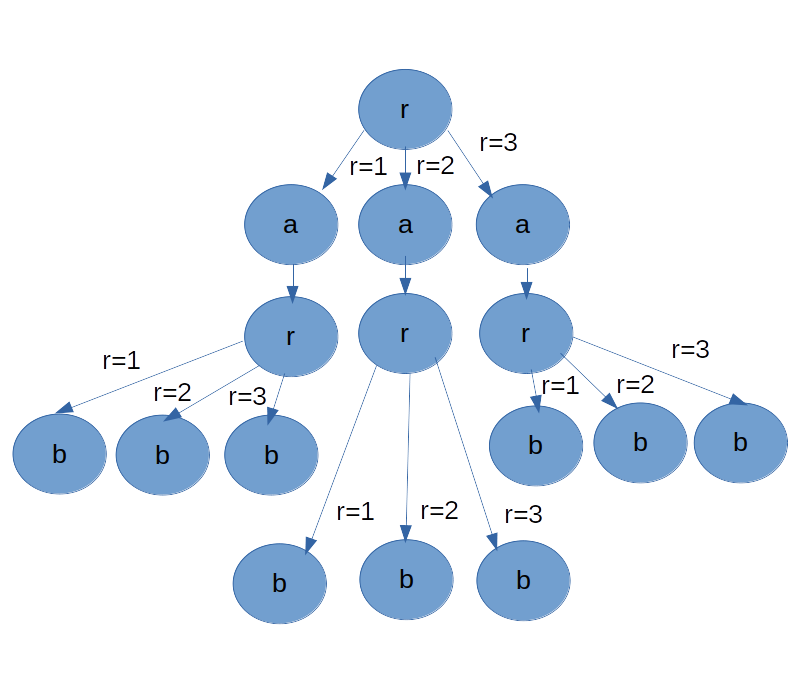
\includegraphics[width=0.7\linewidth]{Graphics/Neigh-Tree}
	\caption{Árbol de vecindad asociado a $rarb$.}
	\label{fig:neigh-tree}
\end{figure}

Cada rama del árbol representa un conjunto de soluciones vecinas. Por ejemplo, en la figura \ref{fig:neigh-tree}, la rama más a la izquierda representa todas las posibles soluciones en las que el cliente se escoge de la primera ruta y se inserta también en la primera ruta.

A partir del árbol que representa a una vecindad para una solución, es posible contar la cantidad de vecinos y es posible asignarle a cada vecino un número natural \cite{Hector}. De esta manera, explorar una vecindad se reduce a seleccionar elementos de los $n$ primeros números. En una exploración exhaustiva se seleccionan todos los números mientras que en una aleatoria se selecciona sólo un conjunto de ellos. Usando esta idea, las estrategias de exploración se definen como iteradores que generan un número, calculan cuál es la solución que le corresponde y retornan esta solución en forma de lista de operaciones.

El Árbol de Vecindad permite explorar vecinos. Para cada vecino se necesita conocer su costo y en la siguiente sección se muestra cómo se pueden obtener estos costos mediante un Grafo de Evaluación.

\section{Grafo de Evaluación}\label{1-JJ}
Para resolver un VRP utilizando búsqueda local, es necesario obtener el costo de cada vecino. Los algoritmos de búsqueda local obtienen un vecino a partir de pequeñas modificaciones de la solución actual. Calcular el costo del vecino evaluando la solución en su totalidad suele ser menos eficiente que calcular la variación del costo debido a las operaciones. Por eso, al programar estos algoritmos, es conveniente determinar la manera más eficiente de evaluar vecinos con la menor cantidad de operaciones posibles. 

Por ejemplo, en CVRP, al eliminar un cliente de una ruta sólo es necesario calcular la nueva distancia a partir de la eliminación, y modificar la carga que debe tener el vehículo a lo largo de la ruta. Algo similar ocurre cuando se inserta un cliente.

Si se desea obtener el costo de un vecino con la menor cantidad de operaciones posible, para cada problema y cada operación del criterio de vecindad, se debe programar sus diferencias. Esto puede variar mucho de un problema a otro por lo que calcular el costo de un vecino, para cada variante de VRP es un trabajo distinto y necesita una implementación diferente.

Por ejemplo, en CVRP sólo se debe actualizar la distancia recorrida y la capacidad restante del vehículo, pero en un problema con \textit{backhaul} hay que verificar también si no se incumple la restricción de que todos los clientes de tipo A se visiten antes de los de tipo B.  

Este es, precisamente, uno de los motivos por el que resolver un Problema de Enrutamiento de Vehículos requiere tiempo de desarrollo humano, al tener que programar cómo calcular el costo de los vecinos para cada nuevo problema. En \cite{JJ} se propone un mecanismo que permite calcular el costo de cualquier vecino, a partir, únicamente, del código que calcula el costo de una solución inicial. Esto se hace a través de un Grafo de Evaluación que se expone a continuación.

El Grafo de Evaluación es una estructura que permite almacenar las operaciones realizadas durante la evaluación de una solución. En este grafo hay tres tipos de nodos:

\begin{itemize}
	\item Nodos que representan los elementos de la solución (clientes, depósitos).
	\item Nodos que representan variables y mantienen sus valores (como el costo total). Estos se denominan nodos acumuladores.
	\item Nodos que representan las operaciones involucradas en una evaluación (aumentar valor, disminuir valor). Estos se denominan nodos operacionales.
\end{itemize}

Para calcular el costo de un vecino a partir de las operaciones que se necesitan para obtenerlo, el grafo se modifica para reflejar las modificaciones que se hicieron sobre la solución. El Grafo de Evaluación permite obtener costos de soluciones vecinas de una solución actual de forma eficiente, ya que garantiza que sólo se recalculen los fragmentos de las nuevas soluciones en los que estas se diferencien de la solución actual.

En las siguientes secciones se muestra cómo construir el grafo y cómo ejecutar operaciones sobre un grafo construido .

\subsection{Creación del grafo}

Para construir el grafo, primero se inicializa con los nodos que representan elementos de la solución. Por ejemplo, en la figura \ref{fig:eval-graph-1} se muestra el grafo inicializado con los nodos que representan los elementos de la solución: $s = [(c_1,c_2), (c_3,c_4)]$. Los nodos \textit{d} representan al depósito y los nodos \textit{$c_i$} a cada cliente. Todas las rutas en el grafo comienzan y terminan con nodos depósito.

Luego, el usuario debe ejecutar el código de evaluación de la variante específica que se quiere resolver y, a partir de este código, se construyen los nodos acumuladores y los nodos operacionales. Por ejemplo, a continuación se muestra el código de evaluación de VRP básico en el que soólo se calcula la distancia recorrida:

\begin{lstlisting}
def-var total-distance as 0
loop for r in solution-routes do
	loop for c in r-clients do
		increment total-distance with distance between r-previous-client and c
	set previous-client as c
return-value total-distance graph
\end{lstlisting}

En la línea 1 se crea un nodo para mantener el valor del costo total y en la línea 4 se crean los nodos que aumentan el valor de la distancia total. Cómo programar códigos de evaluación se explicará detalladamente en la sección \ref{2-eval}.

\begin{figure}
	\centering
	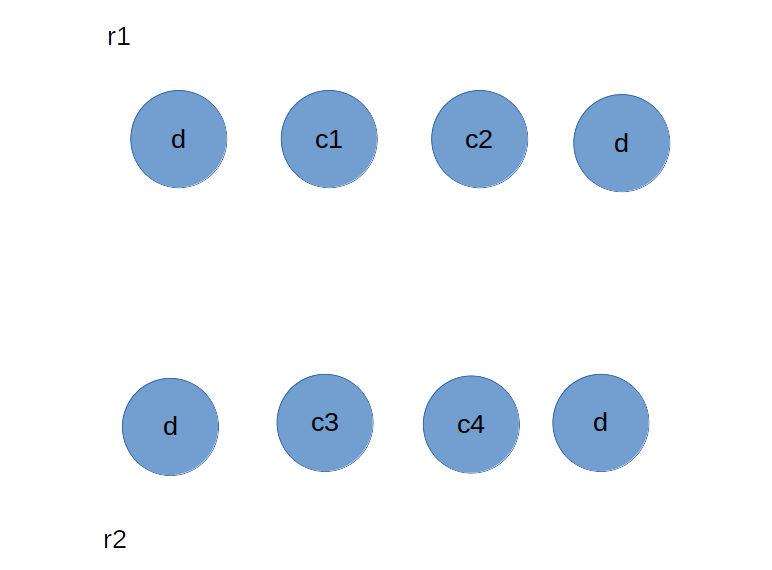
\includegraphics[width=0.9\linewidth]{Graphics/graph-init}
	\caption{Nodos que representan elementos de la solución $s_1$ de VRP básico.}
	\label{fig:eval-graph-1}
\end{figure}

Cuando se ejecuta el código de evaluación a la solución con la que se inicializó el grafo de la figura \ref{fig:eval-graph-1}, se le agregan a este los nodos operacionales y acumuladores. Entonces se obtiene el grafo representado en la figura \ref{fig:eval-graph-2}. El nodo \textit{cost} almacena el costo total de la solución y los nodos con símbolo \textit{+} son nodos operacionales que toman como entrada dos nodos clientes (o depósito) y adicionan al nodo de costo total la distancia entre ellos.

\begin{figure}
	\centering
	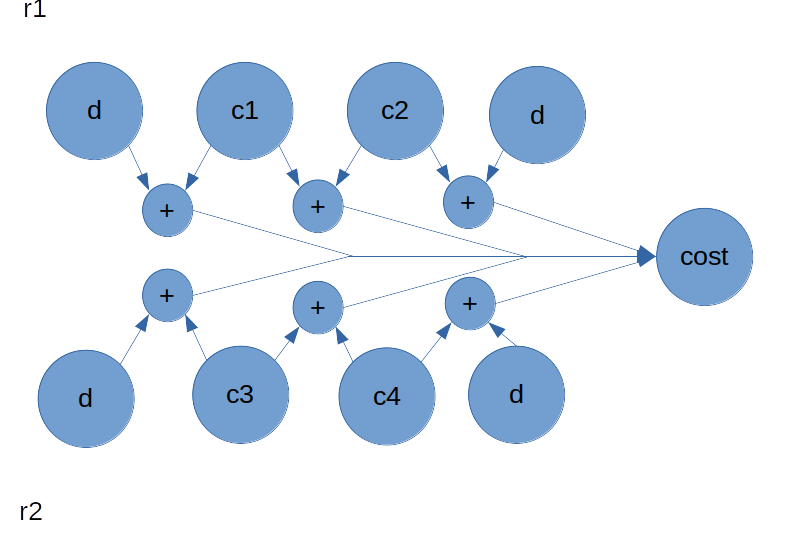
\includegraphics[width=0.9\linewidth]{Graphics/eval-graph-2}
	\caption{Grafo de evaluación que representa la solución $s1$ de VRP básico.}
	\label{fig:eval-graph-2}
\end{figure}

\subsection{Modificación del grafo}
Una vez construido el grafo, las modificaciones que se le realizan se definen mediante operaciones elementales (como eliminar o insertar cliente). Cuando se agregan o eliminan nodos que representan elementos de la solución, se modifican todos los nodos operacionales que dependen de ellos. Estos nodos operacionales tienen asociadas funciones para ejecutarse y para deshacerse. 

Por ejemplo, retirar el cliente $c1$ del grafo representado en \ref{fig:eval-graph-2} (VRP clásico) provoca que los dos nodos \textit{+} que utilizan dicho cliente como entrada deshagan sus operaciones, y al mismo tiempo, se crea y ejecuta un nuevo nodo \textit{+} que recibe como entrada $d$ y $c2$. Luego, insertar a $c1$ al final de la ruta $r2$ se deshace la operación el nodo \textit{+} que recibe como entrada a $c4$ y $d$ mientras se crean y ejecutan dos nodos \textit{+} nuevos, uno recibiendo de entrada a $c4$ y $c1$ mientras que el otro a $c1$ y $d$. El resultado de estas dos operaciones se muestra en \ref{fig:eval-graph-4} y es, precisamente, el grafo resultante de aplicar al grafo de la figura \ref{fig:eval-graph-2}, el criterio \texttt{mover un cliente a cualquier ruta en cualquier posición}, formado por las siguientes operaciones:

\begin{itemize}
	\item Seleccionar ruta \texttt{r1}.
	\item Seleccionar cliente \texttt{c1} de la posición \texttt{2} de la ruta \texttt{r1}.
	\item Seleccionar ruta \texttt{r2}.
	\item Insertar cliente \texttt{c1} en la posición texttt{3} de la ruta \texttt{r2}.
\end{itemize}

Nótese que luego de aplicar los métodos \texttt{evaluate} y \texttt{undo} correspondientes el nodo $cost$ tiene almacenado el costo de la solución resultante luego de aplicar el criterio \texttt{mover cliente a una posición aleatoria en una ruta aleatoria}. Para encontrar el costo de la nueva solución sólo fue necesario analizar y modificar los nodos en que el grafo de la solución nueva se diferencia de la solución anterior y no todo el grafo. En esto se basa la evaluación \textit{eficiente} del Grafo de Evaluación.

\begin{figure}
	\centering
	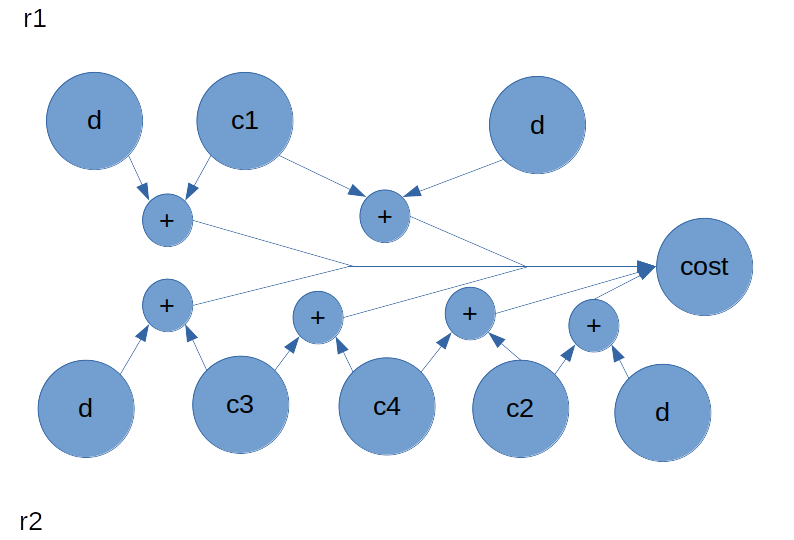
\includegraphics[width=0.9\linewidth]{Graphics/eval-graph-4}
	\caption{Grafo de evaluación que representa la solución $s1$ de VRP básico luego de mover el cliente $c2$}
	\label{fig:eval-graph-4}
\end{figure}

Para explorar una vecindad a partir de un criterio es necesario (además de generar y evaluar soluciones) decidir e implementar estrategias de exploración y de selección. A partir de combinaciones de diferentes estrategias se pueden realizar exploraciones con distintos resultados. Esto se trata en la siguiente sección.

\section{Combinación de estrategias de exploración y selección.}\label{1-Heidy}
Las exploraciones de las vecindades obtienen diferentes resultados en dependencia de las estrategias de exploración y de selección que se utilice. Por ejemplo, a partir de una solución actual y un criterio, se puede explorar una vecindad con una búsqueda exhaustiva y mejora aleatoria o con una búsqueda aleatoria y primera mejora. En ambos casos se pueden encontrar soluciones distintas. Programar cada combinación de estas estrategias demanda tiempo de trabajo humano.

En \cite{Heidy} se propone una herramienta que permite generar funciones de exploración a partir de un criterio, una estrategia de selección y una de exploración. Las posibles estrategias se definen como clases y usando instancias de estas clases se puede generar una función de exploración que se comporte de acuerdo a las instancias recibidas. La generación de cada porción del código se logra utilizando funciones genéricas, en particular los métodos \texttt{after} \cite{Lisp2006}.

La función de exploración resultante recibe el problema que se quiere resolver junto con una solución actual, ejecuta la exploración y retorna un vecino de acuerdo al criterio de selección. Si ninguna solución explorada cumple con la estrategia de selección, se retorna \texttt{nil}. 

En \cite{Heidy}, para realizar la exploración, se utilizaban ciclos que hacían poco flexible incorporar nuevas estrategias. Con el Árbol de vecindad es posible crear cualquier exploración y diseñar estrategias de búsqueda más complejas. Además, en \cite{Heidy} tampoco se usa el Grafo de Evaluación por lo que la cantidad de problemas que podían ser evaluados era limitada. En este trabajo se combinan el Árbol de Vecindad y el Grafo de Evaluación junto con el generador de funciones de exloración. Esto permite resolver cualquier problema que se pueda evaluar en el grafo, con cualesquiera combinaciones de estrategias de exploración y selección. El siguiente capítulo expone cómo se unen todas estas herramientas.






























\chapter{Propuesta de solución}\label{chapter:Solution}

La implementación del sistema está dividida en cuatro módulos: Núcleo, trabajo con vecindades, evaluación de soluciones y generador de funciones de exploración.

\begin{itemize}
	\item Núcleo (\texttt{Core}): En este módulo se implementan las clases a partir de las cuales se pueden describir las soluciones y criterios de vecindad para Problemas de Enrutamiento de Vehículos.
	\item Trabajo con vecindades (\texttt{Neigh}): Se implementa el Árbol de Vecindad a partir del cual se genera soluciones con distintas formas de exploración de vecindades.
	\item Evaluación de soluciones (\texttt{Eval}): Se implementa el grafo de evaluación con el que se obtiene el costo de soluciones vecinas a partir de cómo se evalúa una solución.
	\item Generador de funciones de exploración (\texttt{Generator}): Este módulo contiene el código que permite generar funciones de exploración para combinar estrategias de exploración y selección.
\end{itemize}

Estos cuatro módulos ya existían antes de que se desarrollara el presente trabajo. En las secciones siguientes se describen los detalles de cada uno de estos módulos, cómo se combinaron y qué modificaciones se le hizo a cada uno para implementar esta tesis. En la sección \ref{2-core} se describe el módulo \texttt{core}. En la sección \ref{2-neigh} se describe el módulo \texttt{neigh}. En la sección \ref{2-eval} se describe el módulo \texttt{eval}. Por último, en la sección \ref{2-generator} se describe el módulo \texttt{generator}

\section{Vrp-core}\label{2-core}

En el módulo \textit{core} se definen funciones para inicializar el sistema, así como implementaciones de algoritmos de búsqueda local que utilizan funciones del sistema para explorar vecindades.

También se define un conjunto de clases que permiten describir soluciones para un Problema de Enrutamiento de Vehículos. A partir de esas soluciones se construye el grafo de evaluación.

También se definen clases que permiten definir los datos necesarios para resolver problemas específicos. Por ejemplo, para CVRP es necesaria la demanda de cada cliente y la matriz que guarda la distancia entre cada par de clientes. Para el Problema con backhaul, se define también una lista que guarda los tipos de cada cliente. En el capítulo \ref{chapter:Tutorial} se discute cómo ampliar el sistema para definir otras variantes de VRP.

Además, en este módulo se tiene clases que representan las operaciones que conforman los criterios de vecindad (como seleccionar ruta o insertar cliente).

Para el desarrollo de esta tesis, no se añadió código al módulo \textit{core}. Por el contrario, se desecharon secciones de código que quedaron obsoletas. Por ejemplo, en la versión anterior se utilizaba algo llamado \textit{solución de trabajo}, que era una copia de la solución actual sobre la que se realizaban las modificaciones para evaluar vecinos eficientemente. Como en esta tesis las evaluaciones se hacen mediante el Grafo de Evaluación, las \textit{soluciones de trabajo} quedan obsoletas. En la versión anterior se tenía también unos mecanismos con los que se exploraba vecindades, que al incorporar el Árbol de vecindad fueron desechados.

Una vez definidas las clases que permiten crear una solución, definir características de un problema, y definir un problema, es posible construir un Árbol de Vecindad. Esto se hace en el módulo \texttt{neigh}.

\section{Vrp-neigh}\label{2-neigh}
En este módulo se define el Árbol de Vecindad como una clase que se construye a partir de un problema, una solución y un criterio de vecindad. 

El Árbol de Vecindad permite crear iteradores (o generadores) de soluciones. La función que se usa para crear el iterador depende del tipo de exploración que se desee. Por ejemplo, \texttt{exhaustive-exploration} para la exploración exhaustiva o \texttt{random-exploration} para la exploración aleatoria. Cada vez que se ejecuta un iterador, se obtiene la lista de operaciones que se aplican a la solución actual para generar un vecino, o \texttt{nil} en caso de que no queden vecinos por analizar. Esta condición varía según el tipo de exploración. Por ejemplo, para la exploración exhaustiva se generan todas las soluciones de la vecindad, mientras que en una aleatoria se genera una cantidad predefinida de vecinos. 

En el trabajo original donde se desarrolló este módulo, las clases se definían de manera distinta a como se definen en el módulo \texttt{core}. Por tanto, en el presente trabajo se modificaron las definiciones de clases del módulo \texttt{neigh} para volverlas consistentes con el resto del sistema. También se agregó la función \texttt{random-exploration} para obtener el iterador de exploración aleatoria.

A partir del Árbol de Vecindad se obtienen iteradores que generan vecinos en forma de lista de operaciones. Al aplicar estas operaciones sobre la solución actual se obtiene una solución cuyo costo se puede calcular utilizando el Grafo de Evaluación.

\section{Vrp-eval}\label{2-eval}
En esta sección se implementa el Grafo de Evaluación, que como se presentó en la sección \ref{1-JJ}, tiene tres tipos de nodos: Nodos que representan los elementos de la solución (clientes, depósitos), nodos acumuladores (como el costo total), y nodos operacionales (aumentar valor, disminuir valor). 

El grafo contiene los siguientes elementos:

\begin{itemize}
	\item Una copia de la solución actual.
	\item Una lista con los nodos del grafo.
	\item Una correspondencia entre cada elemento de la solución y el nodo del grafo que lo representa.
	\item Una correspondencia entre los nodos acumuladores y las variables a las que representan.
	\item El valor del costo total de la solución.
\end{itemize}

Para incorporar este módulo al sistema hubo que reimplementarlo prácticamente desde cero. En su versión anterior, el código del grafo de evaluación estaba aislado del módulo \texttt{core} y, por tanto, este grafo no se podía construir a partir de las clases para describir soluciones que utiliza el sistema. Con el desarrollo de este trabajo se crearon métodos y clases de inicialización, construcción y modificación de grafo compatibles con las clases de \texttt{core}.

Para inicializar un grafo sólo es necesaria la solución actual. La inicialización consiste en convertir los elementos de la solución (clientes, depósitos, vehículos) en los nodos que los representan.

Para terminar de construir el grafo, se debe definir y ejecutar el código de evaluación de la solución inicial a partir de funciones definidas en el sistema. Algunos ejemplos de estas funciones son:

\begin{itemize}
	\item \texttt{def-var}: Recibe un nombre y un valor inicial. Inicializa un nuevo nodo acumulador y se lo hace corresponder con el nombre recibido.	
	\item \texttt{increment-distance}: Recibe dos clientes, una variable asociada a un nodo acumulador y la matriz de distancia. Crea y evalúa un nodo operacional que incrementa el valor almacenado en el nodo correspondiente a la variable en una cantidad igual a la distancia entre los clientes.
	\item \texttt{decrement-demand}: Recibe un cliente y una variable asociada a un nodo acumulador. Crea y evalúa un nodo operacional que recibe el cliente y decrementa el valor del nodo correspondiente a la variable en una cantidad igual a la demanda del cliente.
	\item \texttt{increment-value}: recibe dos variables. Incrementa el valor del nodo asociado a la segunda variable en una cantidad igual al valor del nodo asociado a la primera variable.
	\item \texttt{apply-penalty}: Recibe dos variables y un factor de penalización. Crea y evalúa un nodo operacional que recibe el nodo asociado a la primera variable y, en caso de que este tenga valor negativo, aumenta el valor del nodo asociado a la segunda variable en una cantidad que depende del factor de penalización.
	\item \texttt{return-value}: Recibe una variable y marca su nodo asociado como el nodo que contiene el costo total de la solución. A partir del punto en que se invoca, la propiedad \textit{output} (salida o costo total) del grafo referencia a este nodo.
\end{itemize}

Todas las funciones de construcción de grafo reciben también como parámetro la instancia del grafo sobre el que se está trabajando. En el capítulo \ref{chapter:Tutorial} se discutirá la ampliación del sistema con nuevos métodos. 

A continuación se muestra el pseudo-código que evalúa una solución de CVRP.

\begin{lstlisting}
def-var total-distance (initial-value = 0)
loop for r in solution-routes do
	def-var route-distance (initial-value = 0)
	def-var route-capacity (initial-value = vehicles-capacity)	
	loop for c in r-clients do
		increment route-distance in distance between r-previous-client c 
		decrement route-demand in client-capacity	
	set r-previous as c
	increment total-distance in route-distance
	apply-penalty in total-distance with route-capacity
return-value total-distance

\end{lstlisting}

En las líneas 1 se usa def-var para inicializar, y asociar a su respectivos nodos, la variable que almacenan el costo total de la solución. Luego se analizan las rutas de la solución. Por cada ruta se definen, y asocian a sus respectivos nodos, variables que almacena el costo (línea 3) y la capacidad restante de la ruta (líneas 4). A continuación se analizan los clientes de la ruta actual. Se incrementa el valor del nodo asociado al costo de la ruta en una cantidad igual a la distancia del cliente actual y el cliente previo (el cliente previo inicial de la ruta es el depósito)(línea 6). También se decrementa el valor del nodo asociado a la capacidad de la ruta en una cantidad igual a la demanda del cliente actual (línea 7) Una vez se analiza una ruta, se aumenta el valor del nodo asociado al costo total de la solución en una cantidad igual al costo de esta ruta (línea 8) y se penaliza el nodo de costo total en caso de ser necesario (línea 9). Finalmente se declara como nodo salida al nodo asociado a la variable de distancia total (línea 10).

En su versión anterior, el módulo \texttt{eval} tampoco era compatible con las clases de \texttt{core} que describen operaciones de vecindad. Para aplicar y deshacer en el grafo las operaciones de vecindad que utiliza el sistema se implementaron las funciones \texttt{do-core-operations} y \texttt{undo-core-operations}.

\texttt{Do-core-operations} recibe una lista de operaciones y el grafo sobre el cual estas se ejecutan. Las operaciones se hacen en orden. Los nodos que representan elementos de la solución se insertan o eliminan del grafo y los nodos operacionales que dependan de ellos se ejecutan o deshacen. Por ejemplo, dado el grafo representado en la figura \ref{fig:eval-graph-5}, al ejecutar el siguiente código:



\begin{lstlisting}
do-core-operations (graph ((op-select-client 1 from route 1)
										(op-insert-client 1 to route 3 in 2))
\end{lstlisting}

Se obtiene el grafo representado en \ref{fig:eval-graph-4}. En este punto, la propiedad \textit{output} del grafo (Que en este caso hace referencia al nodo \textit{cost}) tiene el costo total de la nueva solución.

Para deshacer operaciones que se hicieron previamente en un grafo se ejecuta la función \texttt{undo-core-operations}. Por ejemplo, al ejecutar el siguiente código sobre el grafo representado en la figura \ref{fig:eval-graph-6}:



\begin{lstlisting}
undo-core-operations (graph ((op-select-client 1 from route 1)
											(op-insert-client 1 in route 3 in 2))
\end{lstlisting}

Se obtiene nuevamente el grafo representado por \ref{fig:eval-graph-2} y el valor almacenado en \textit{cost} vuelve a ser el costo total de la solución original.

El Grafo de Vecindad en la forma que se implementó, no es capaz de evaluar vecinos de variantes de VRP que tengan ciertas características y sobre esto trata la siguiente sección.

\begin{figure}
	\centering
	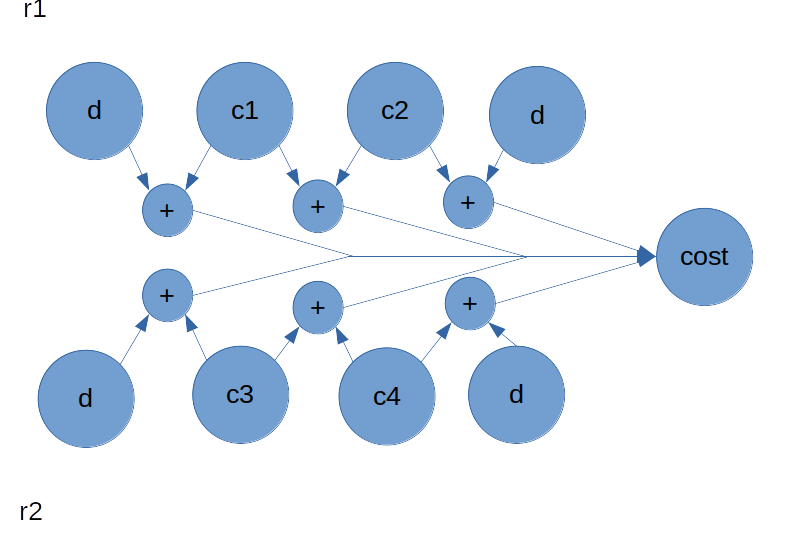
\includegraphics[width=0.9\linewidth]{Graphics/eval-graph-2}
	\caption{Grafo de evaluación que representa la solución $s1$ de VRP básico.}
	\label{fig:eval-graph-5}
\end{figure}

\begin{figure}
	\centering
	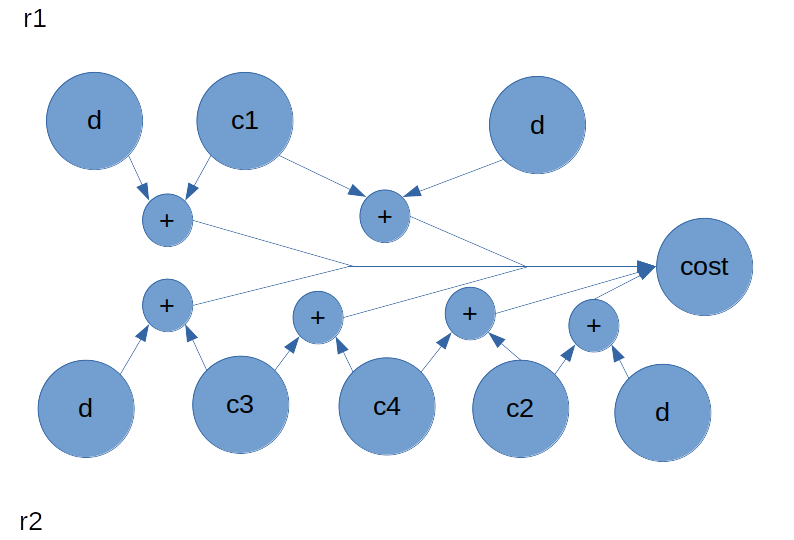
\includegraphics[width=0.9\linewidth]{Graphics/eval-graph-4}
	\caption{Grafo de evaluación que representa la solución $s1$ de VRP básico luego de mover el cliente $c2$}
	\label{fig:eval-graph-6}
\end{figure}

\subsection{Limitaciones}

En esta sección se describen las variantes de VRP en las cuales no es posible evaluar vecinos mediante el Grafo de evaluación tal y como se ha implementado en el presente trabajo. Para ello se tomará como ejemplo el Problema de Enrutamiento de Vehículos con recogidas y entregas. 

En el Problema de Enrutamiento de Vehículos con recogidas y entregas a cada cliente se le entrega pero también se le recogen productos. En este caso, además, el cliente es visitado una sola vez, por lo que la recogida y la entrega se realizan al mismo tiempo y con el mismo vehículo. Como consecuencia, es posible que se incumpla la restricción de capacidad sin que la cantidad total de producto que se debe entregar a cada cliente de la ruta exceda la capacidad del vehículo. Por ejemplo, puede que el exceso de carga lo provoque la recogida de productos al atender a un cliente durante el recorrido de la ruta.

En esta variante se penaliza el exceso de carga al visitar cada cliente de la ruta, al contrario de como se hace en la evaluación de una solución de CVRP donde la penalización se realiza al finalizar el recorrido de cada ruta. Las soluciones vecinas de los problemas en los que la función objetivo incluye penalizaciones durante el recorrido de una ruta no se pueden evaluar con el grafo que se implementó en este trabajo \cite{JJ}.

A pesar de que se puede obtener un grafo de evaluación y el resultado de la evaluación de la solución inicial para VRPPD, no sucede lo mismo con las soluciones vecinas de esta. Por ejemplo, al extraer un cliente no se conoce el valor que contenía la capacidad restante de su ruta cuando en la evaluación de la solución inicial se visitó a ese cliente y, por tanto, no se puede revertir la penalización que se pudo haber aplicado en ese momento.

En general no es posible evaluar vecinos en problemas en los que se realicen operaciones durante el recorrido de una ruta que dependan de variables que se modifiquen durante ese recorrido \cite{JJ}.

Una vez que se definen funciones que generan y evalúan soluciones, sólo resta utilizarlas en exploraciones de vecindades. Este tema se aborda en la siguiente sección.

\section{Vrp-generator}\label{2-blueprint}
Una vecindad se puede analizar con distintas estrategias de exploración y selección. Cada vez que se combina una estrategia de exploración con una de selección se obtiene una manera diferente de analizar la vecindad. A cada una de estas combinaciones, en este trabajo se les llama función exploradora de la vecindad. Programar estas funciones exploradoras es un proceso con alto consumo de tiempo de trabajo humano. En \cite{Heidy} se propone un mecanismo para automatizar la creación de funciones exploradoras a partir de cualesquiera estrategias de exploración y selección, con un esfuerzo mínimo. Esto significa que ya no es necesario programar todas las funciones de exploración diferentes, lo cual agiliza el tiempo de desarrollo. Para esto, se utilizan las ventajas del Sistema de Objetos de Common Lisp (CLOS), en particular las combinaciones de métodos y la facilidad que brinda el lenguaje para generar código fuente en tiempo de ejecución.

Las posibles estrategias de exploración y selección se representan como clases y los criterios de vecindad mediante una lista de operaciones. En \cite{Heidy} se tiene una un mecanismo que recibe una estrategia de exploración, una de selección y un criterio, y devuelve una función que dada una solución explora la vecindad correspondiente a esas entradas.

La versión del módulo \texttt{generator} que se hizo en \cite{Heidy} utilizaba en las funciones de exploración que se generaban, elementos de \texttt{core} que con este trabajo quedaron obsoletos. Por tanto, parte de los mecanismos desarrollados en \cite{Heidy} también quedaron obsoletos.

En la versión anterior las vecindades se exploraban con cadenas de ciclos que mezclaban las operaciones. En el presente trabajo, esto se hace con un único ciclo que genera soluciones a partir del iterador del Árbol de Vecindad. Por otro lado, los vecinos se evaluaban mediante \textit{soluciones de trabajo} y esto ahora se hace mediante el Grafo de Evaluación.

En este trabajo se define un nuevo generador de funciones que utiliza un Árbol de Vecindad y que, además, en lugar de recibir una solución, ahora reciben un Grafo de Evaluación.

En \cite{Heidy} el código de una función de exploración (y por tanto, el código que se genera a partir de la función generadora) está dividido en 5 regiones comunes para cualquier exploración:

\begin{itemize}
	\item Inicializaciones de variables.
	\item Ciclos que definen cómo realizar la exploración (dependen del criterio).
	\item Instrucciones que se ejecutan dentro de los ciclos.
	\item Instrucciones que se ejecutan fuera de los ciclos.
	\item Valores que se retornan.
\end{itemize}

El siguiente pseudo-código muestra un ejemplo de función exploradora para el criterio \textit{mover cliente de posición dentro de su ruta} con estrategia de exploración exhaustiva y con selección de mejor vecino. Esta función recibe una solución (\texttt{solution}) como argumento.

\begin{lstlisting}
set wc as working-copy of solution
set ops-list as nil
set current-cost as 0
set best-cost as 0
set best-neighbor as nil
set result-solution as nil

loop foreach route r:
	loop foreach client c:
		loop foreach pos p:
			
			set current-ops-list as (select-route-r,
												 select-client-c,
												 insert-client-c-in-route-r-in-position-p)
			set current-cost as apply-operations(wc current-ops-list)
			if (current-cost < best-cost) then:
				set best-neighbor as current-ops-list
				set best-cost as current-cost
				
if (best-neighbor exists) then
	set result-solution as operations best-neighbor applied over solution
	
return result-solution


\end{lstlisting}

En las líneas 1-6 seinicializan las variables necesarias. En las líneas 8-10 se crean los ciclos que definen cómo realizar la exploración, por cada operación del criterio se hace un ciclo. Las líneas 12-18 contienen el código dentro de los ciclos, se obtiene el costo actual a partir de la \textit{solución de trabajo} y en caso de ser menor que el actual mejor costo, se actualiza \texttt{best-cost} y \textit{best-neighbor}. Las líneas 20-21 tienen el código fuera de los ciclos, en caso de haberse encontrado un mejor vecino, se aplican sus operaciones sobre la solución actual para obtener la nueva solución. La línea 23 retorna la solución encontrada.

En este trabajo, la sección de los ciclos que definen cómo realizar la exploración se cambia por un único ciclo cuya condicional depende de la estrategia. El sigiente pseudo-código muestra la implementación del ejemplo anterior generado por el sistema desarrollado en esta tesis. Esta función recibe un grafo (\texttt{graph}) como parámetro.

\begin{lstlisting}
set neigh-tree as build-neigh-tree with criteria and graph-solution
set generator as exhaustive-exploration(neigh-tree)
current-ops-list as funcall(generator)

set best-cost as 0
set best-neighbor as nil

cicle while (current-ops-list exists)
			
			do-core-operations (current-solution graph)
			set current-cost as output of graph
			undo-core-operations (current-solution graph)
			if (current-cost < best-cost) then:
				set best-neighbor as current-ops-list
				set best-cost as current-cost
			set current-ops-list as funcall(generator)

if (best-neighbor exists) then
	do-core-operations best-neighbor over graph

return graph-current-solution
\end{lstlisting}

En la línea 8 se sustituye el código de la región de los ciclos por un único ciclo que se ejecutará mientras se cumpla su condición (en este caso, que el generador retorne un vecino). Además, la función ahora genera los vecinos a partir de un Árbol de Vecindad y en lugar de recibir una solución como argumento, recibe el grafo asociado a esa solución mediante el cual se obtiene el costo de los vecinos.

En este capítulo se explicaron las características de cada módulo de este trabajo. El siguiente capítulo explica paso a paso cómo utilizar el sistema para resolver variantes de VRP. 











\chapter{Método de uso}\label{chapter:Tutorial}

Este capítulo explica los pasos que debe seguir un usuario para resolver variantes de VRP utilizando el sistema que se implementó en este trabajo. Esto se hará a través de un ejemplo de resolución de un problema CVRP arbitrario.

En la sección \ref{4-problem} se define el problema. En la sección \ref{4-solution} se construye el grafo de evaluación y la solución inicial. En la sección \ref{4-generator} se generan las funciones de exploración. En \ref{4-union} se presenta el código completo.

\section{Definición del problema}\label{4-problem}

El primer paso para resolver un VRP usando este sistema, es definirlo usando las clases que lo representan a él y a sus características. Esto se mostrará a través de un ejemplo de resolución de un CVRP con seis clientes. En este caso, se debe crear un objeto de tipo \texttt{basic-cvrp-client} (cliente con demanda) por cada cliente, uno de tipo \texttt{basic-depot} (depósito) y una matriz de distancias de tamaño $6x6$. 

El siguiente código se usa para definir el problema.

 \begin{lstlisting}
(defparameter c1 (basic-cvrp-client 1 1))
(defparameter c2 (basic-cvrp-client 2 1))
(defparameter c3 (basic-cvrp-client 3 4))
(defparameter c4 (basic-cvrp-client 4 3))
(defparameter c5 (basic-cvrp-client 5 2))
(defparameter c6 (basic-cvrp-client 6 1))

(defparameter d0 (basic-depot))

(defparameter dist-mat #2A((0 1 2 3 4 5 6)
										(1 0 5 2 1 3 2)
										(2 5 0 2 2 2 2)
										(3 2 2 0 1 2 1)
										(4 1 2 1 0 2 3)
										(5 3 2 2 2 0 1)
										(6 2 2 1 3 1 0)))

(defparameter problem (basic-cvrp-problem 
										:id 1 
										:clients (list c1 c2 c3 c4 c5 c6)
										:depot d0 
										:distance-matrix dist-mat 
										:capacity 20))
\end{lstlisting}

En las líneas 1 a 6 se definen los clientes, estos reciben dos parámetros, \textit{id} y \textit{demanda} respectivamente. Los vehículos se definen en las líneas 8 y 9, reciben también dos parámetros \textit{id} y \textit{capacidad} respectivamente. Luego se declara el depósito (línea 11), la matriz de distancias (línea 13) y se crea la instancia del problema (línea 21).

Una vez se definió el problema, se debe crear una solución inicial como se muestra en la siguiente sección.

\section{Solución inicial y Grafo de Evaluación}\label{4-solution}

La solución inicial se utiliza para construir e inicializar el grafo. En el caso de CVRP una solución está formada por una lista de rutas que son instancias de la clase \texttt{route-for-simulation}. El siguiente código muestra cómo se crea una solución:


\begin{lstlisting}
(defparameter r1 (route-for-simulation 
							:id 1
							:vehicle (cvrp-vehicle 1 20) 
							:depot d0
							:clients (list c1 c2 c3 (clone d0))
							:previous-client (clone d0)))
(defparameter r2 (route-for-simulation 
							:id 2 
							:vehicle (cvrp-vehicle 2 20)
							:depot d0
							:clients (list c4 c5 c6 (clone d0))
							:previous-client (clone d0)))

(defparameter s1 (basic-solution
							:id 1 
							:routes (list r1 r2)))
\end{lstlisting}

Las rutas se definen como instancias de la clase \texttt{rute-for-simulation} (líneas 1 y 7). Esta clase hereda de la clase \texttt{basic-route} y la extiende con la propiedad \textit{previous-client}. Esta propiedad se inicializa con una referencia al depósito a partir de la cual se crea el primer nodo de la ruta en el grafo de evaluación y simplifica la implementación del código de evaluación de la solución. Nótese que las rutas del grafo de evaluación comienzan y terminan en el depósito que se debe clonar para tener, en cada posición, nodos distintos.

Luego se debe inicializar el grafo con la función \texttt{init-graph}.

\begin{lstlisting}
(defparameter graph (init-graph s1))
\end{lstlisting}

Una vez que el grafo está inicializado, se le deben agregar las operaciones y nodos que mantienen valores. Esto se consigue mediante el código de evaluación de la solución inicial.

\begin{lstlisting}
(def-var total-distance 0 graph)
(loop for r in (routes s1) do
	(def-var route-distance 0 graph)
	(def-var route-demand (capacity (vehicle r)) graph) 
	(loop for c in (clients r) do 
		(increment-distance (previous-client r) c route-distance dist-mat graph)
		(decrement-demand c route-demand graph) 
		(setf (previous-client r) c)
	(increment-value total-distance route-distance graph)
	(apply-penalty route-demand total-distance 10 graph)
(return-value total-distance graph))
\end{lstlisting}

En la línea 1 se usa \texttt{def-var} para inicializar la variable que almacena el costo total de la solución. Luego se analizan las rutas de la solución. Por cada ruta se define una variable nueva que almacena su costo (línea 3) y otra que almacena la capacidad restante de su vehículo (línea 4). Entonces se analizan los clientes de la ruta actual. Se incrementa el costo de la ruta en una cantidad igual a la distancia del cliente actual y el cliente previo (el cliente previo inicial de la ruta es el depósito), y se disminuye la capacidad del vehículo en una cantidad igual a la demanda del cliente (líneas 6 y 7 respectivamente). Después de analizar cada ruta se aumenta el costo total de la solución en una cantidad igual a los costos de las mismas y se aplica penalización en caso de que un vehículo haya alcanzado una capacidad restante negativa (líneas 9 y 10). Finalmente se retorna la distancia total.

La siguiente sección ejemplifica cómo se generan las funciones de exploración a partir de criterios de vecindad y estrategias de exploración y selección.

\section{Generación de funciones de exploración}\label{4-generator}

Una vez que se tiene el grafo de evaluación de una solución inicial, para resolver el problema con una búsqueda local se debe definir cómo explorar la vecindad.

Las estrategias de exploración y selección se definen como clases cuyas instancias se pasan como parámetros a la función generadora. Se utilizan métodos que reciben estas instancias y generan código a partir de especializaciones de los tipos de los argumentos recibidos.

A continuación se presentan algunas clases que representan estrategias de exploración y selección:\\

\textit{Exploración:}
\begin{itemize}
	\item \texttt{exhaustive-neighborhood-search-strategy}: Exploración exhaustiva.
	\item \texttt{random-neighborhood-search-strategy}: Exploración aleatoria.
\end{itemize}

\textit{Selección:}
\begin{itemize}
	\item \texttt{best-improvement-search-strategy}: Selección de mejor solución.
	\item \texttt{first-improvement-search-strategy}: Selección de primera mejora.
	\item \texttt{random-improvement-with-candidates-selection-strategy}: Selección aleatoria de una mejora entre los elementos de una lista con las mejoras encontradas.
	\item \texttt{random-improvement-selection-strategy}: Selección aleatoria de una mejora en base a una probabilidad.
\end{itemize}

Durante la definición de cada clase se crea un parámetro global que almacena una instancia de su respectiva clase. Por ejemplo, el parámetro \texttt{+exhaustive-search-strategy+} tiene como valor asociado una instancia de \texttt{exhaustive-neighborhood-search-strategy}.

A continuación se define una lista de funciones de exploración para los criterios \textit{mover un cliente dentro de su ruta}, \textit{mover un cliente a cualquier ruta en cualquier posición} e \textit{intercambiar dos clientes de posición}. En todos los casos se hace una búsqueda exhaustiva con selección de mejor vecino.

\begin{lstlisting}
(setf rab (make-neighborhood-criterion 
						`((select-route r1)
						(select-client c1 from r1)
						(insert-client c1 to r1))
						+exhaustive-search-strategy+ 
						+best-improvement+))

(setf rarb (make-neighborhood-criterion 
						`((select-route r1)
						(select-client c1 from r1)
						(select-route r2)
						(insert-client c1 to r2))
						+exhaustive-search-strategy+ 
						+best-improvement+))

(setf rarac (make-neighborhood-criterion 
						`((select-route r1)
						(select-client c1 from r1)
						(select-route r2)
						(select-client c2 from r2)
						(swap-clients c1 c2))
						+exhaustive-search-strategy+ 
						+best-improvement+))

(setf criteria (list rab rarb rarac))

\end{lstlisting}

En este punto es posible invocar la función de metaheurística de Búsqueda de Vecindad Variable y obtener una solución.

\begin{lstlisting}
(setf result (vns-vrp-system problem criteria graph :max-iter 1000))
\end{lstlisting}

La siguiente sección muestra el código completo que soluciona un CVRP con datos ficticios.

\section{Código completo}\label{4-union}

\begin{lstlisting}
(defparameter c1 (basic-cvrp-client 1 1))
(defparameter c2 (basic-cvrp-client 2 1))
(defparameter c3 (basic-cvrp-client 3 4))
(defparameter c4 (basic-cvrp-client 4 3))
(defparameter c5 (basic-cvrp-client 5 2))
(defparameter c6 (basic-cvrp-client 6 1))


(defparameter d0 (basic-depot))

(defparameter dist-mat #2A((0 1 2 3 4 5 6)
										(1 0 5 2 1 3 2)
										(2 5 0 2 2 2 2)
										(3 2 2 0 1 2 1)
										(4 1 2 1 0 2 3)
										(5 3 2 2 2 0 1)
										(6 2 2 1 3 1 0)))

(defparameter problem (finite-fleet-cvrp-problem 
										:id 1 
										:clients (list c1 c2 c3 c4 c5 c6)
										:depot d0 
										:distance-matrix dist-mat 
										:capacity 20))

(defparameter r1 (route-for-simulation 
									:id 1
									:vehicle (cvrp-vehicle 1 20) 
									:depot d0
									:clients (list c1 c2 c3 (clone d0))
									:previous-client (clone d0)))
(defparameter r2 (route-for-simulation 
									:id 2 
									:vehicle (cvrp-vehicle 2 20)
									:depot d0
									:clients (list c4 c5 c6 (clone d0))
									:previous-client (clone d0)))

(defparameter s1 (basic-solution
									:id 1 
									:routes (list r1 r2)))

(defparameter graph (init-graph s1))


(def-var total-distance 0 graph)
(loop for r in (routes s1) do
	(def-var route-distance 0 graph)
	(def-var route-demand (capacity (vehicle r)) graph) 
	(loop for c in (clients r) do
		(increment-distance (previous-client r) c route-distance dist-mat graph)
		(decrement-demand c route-demand graph) 
		(setf (previous-client r) c))
	(increment-value total-distance route-distance graph)
	(apply-penalty route-demand total-distance 10 graph) 
(return-value total-distance graph))


(setf rab (make-neighborhood-criterion 
								`((select-route r1)
								(select-client c1 from r1)
								(insert-client c1 to r1))
								+exhaustive-search-strategy+ 
								+best-improvement+))

(setf rarb (make-neighborhood-criterion 
								`((select-route r1)
								(select-client c1 from r1)
								(select-route r2)
								(insert-client c1 to r2))
								+exhaustive-search-strategy+ 
								+best-improvement+))

(setf rarac (make-neighborhood-criterion 
								`((select-route r1)
								(select-client c1 from r1)
								(select-route r2)
								(select-client c2 from r2)
								(swap-clients c1 c2))
								+exhaustive-search-strategy+ 
								+best-improvement+))

(setf criteria (list rab rarb rarac))

(setf result (vns-vrp-system problem criteria graph :max-iter 10000000000))
\end{lstlisting}

Para resolver otra variante de VRP utilizando el sistema que se implementó en el presente trabajo basta con definir las características del problema y el código de evaluación de la solución inicial. Además, cualquier problema que se defina puede ser explorado con cualquier criterio de vecindad sin importar la cantidad de operaciones que tenga y con cualesquiera combinaciones de estrategias de exploración y selección.

En este capítulo se explicó paso a paso el método de uso del sistema. Sin embargo, este sistema no es capaz de resolver todas las variantes de VRP existentes. El siguiente capítulo explica cómo extenderlo para resolver problemas que actualmente no se pueden representar.









\chapter{Extensibilidad}\label{chapter:Extension}

Con las funcionalidades implementadas hasta el momento, el sistema que se propone puede resolver diversas variantes de VRP. Sin embargo, en algún momento, un usuario necesitará resolver un problema que aún no se pueda representar. En este capítulo se explica cómo extender el sistema para otras variantes.

Para extender el sistema a nuevos problemas se debe crear las clases que lo describen y las funciones que permitan construir su grafo de evaluación a partir de una de sus soluciones. También es posible definir nuevas estrategias de exploración y selección.

En \ref{4-description} se explica cómo extender el módulo \texttt{core}. En \ref{4-eval} se explica cómo extender el módulo \texttt{eval}. En el capítulo \ref{4-generator} se explica cómo extender el módulo \texttt{generator}.

\section{Descripción del problema}\label{4-description}
Para extender el sistema a nuevas variantes de VRP puede ser necesario agregar nuevas clases para representar las características del problema. Cada característica depende de las clases de las que hereda. Además, todas las clases que representan características de problemas son descendientes de su clase base correspondiente. Por ejemplo, un cliente de CVRP (clase \texttt{basic-cvrp-client}) hereda de \texttt{demand-client}, clase que indica que el cliente posee una demanda y de \texttt{basic-client}, la clase base para los clientes (que sólo tiene un identificador).

Definir una nueva clase implica identificar de qué clases debe heredar para satisfacer sus especificaciones y, en caso de ser necesario, crear nuevas clases. Definir un problema nuevo puede implicar la creación de varias clases para representar sus características.

A continuación se ejemplificará cómo crear la clase \texttt{basic-time-windows\\-problem} que representa un Problema de Enrutamiento de Vehículos con vetanas de tiempo (VRPTW) \cite{VRPTW}. En este problema los clientes, además de sus demandas, tienen un período de tiempo en que se pueden visitar, de lo contrario se penaliza la solución. Además, cada vez que un vehículo visita un cliente debe esperar un tiempo determinado (tiempo de servicio).

Para definir el VRPTW es necesario definir nuevos clientes, rutas y el problema. 

Primero se crean clientes que conozcan sus ventanas de tiempo y cuánto demora su servicio. Se definen dos clases:

\begin{itemize}
	\item \texttt{time-windows-client}: Tiene ventana de tiempo.
	\item \texttt{service-time-client}: Consume tiempo al ser atendido. 
\end{itemize}

Una vez definidas estas clases, se crea \texttt{basic-tw-client} que representa un cliente de TWVRP y hereda de:

\begin{itemize}
	\item \texttt{basic-client}
	\item \texttt{demand-client}
	\item \texttt{time-windows-client}
	\item \texttt{service-time-client}
\end{itemize}

Las rutas que existen en el sistema no pueden determinar el momento en que se encuentra su vehículo, por eso se deben definir nuevas rutas que conozcan el tiempo actualmente consumido. Se crea la clase \texttt{route-with-\\time} y la clase \texttt{basic-tw-route} que hereda de \texttt{route-with-time} y \texttt{route-\\for-simulation}.

También debe definirse la clase \texttt{time-problem} para indicar que el problema tiene una matriz de $nxn$ cuyas posiciones guardan los tiempos necesarios para viajar entre clientes. Finalmente es posible definir la clase \texttt{basic-time-windows-problem} para el problema con ventanas de tiempo que hereda de las siguientes clases abstractas:

\begin{itemize}
	\item \texttt{basic-problem} (tiene clientes, depósitos e identificador)
	\item \texttt{distance-problem} (tiene matriz de distancias)
	\item \texttt{capacity-problem} (tiene una capacidad por cada cliente)
	\item \texttt{time-problem} (tiene matriz de tiempos)
\end{itemize}

Junto con las nuevas características, definir problema implica también definir cómo evaluar sus soluciones. Al evaluar una solución para un problema determinado puede hacer falta operaciones que aún no existen. La siguiente sección explica cómo definir nuevas operaciones para el Grafo de Evaluación.

\section{Evaluación}\label{4-eval}

Al definir nuevos problemas, también se debe crear la forma en que sus soluciones se evalúan y, en caso de ser necesario, extender el Grafo de Evaluación para incorporar nuevas características y restricciones. Extender el grafo se traduce en agregar los nuevos nodos y las funciones que se usarán en el código de evaluación.

En esta sección se muestra cómo extender el Grafo de Evaluación para obtener el costo de soluciones de CVRP con una restricción extra que consiste en que cada ruta sólo pude tener un número determinado de clientes.

A continuación se muestra el código necesario para evaluar una solución de este problema. Teniendo ese código, se identifican las funciones y clases que se necesita implementar.

Para evaluar una solución se define una variable por cada ruta que se inicializa con valor $k$ y se decrementa en uno por cada cliente de la ruta. Luego, en caso de tener esta variable valor negativo, se penaliza el costo total de la solución. El código de evaluación de CVRP con rutas limitadas se muestra a continuación:

\begin{lstlisting}

(def-var total-distance 0 graph)
(loop for r in (routes s1) do
	(def-var route-distance 0 graph)
	(def-var route-demand (capacity (vehicle r)) graph) 
	(def-var route-limit k graph)
	(loop for c in (clients r) do
		(increment-distance (previous-client r) c route-distance A-n33-k5-distance-matrix graph)
		(decrement-demand c route-demand graph) 
		(decrement-size c route-limit graph) 
		(setf (previous-client r) c))
	(increment-value total-distance route-distance graph)
	(apply-penalty route-demand total-distance 100 graph) 
	(apply-penalty route-limit total-distance 1000 graph)) 
(return-value total-distance graph))
\end{lstlisting}

En la línea 5 se crea la variable \texttt{route-limit}. En la línea 13 se decrementa en uno el valor de \texttt{route-limit} por cada cliente \texttt{c}. En la línea 17 se penaliza el costo total si \texttt{route-limit} tiene valor negativo. 

Para que este código de evaluación funcione, primero debe definirse la función \texttt{decrement-size} que recibe un cliente y crea un nodo operacional \texttt{decrement-size-node} para conectar el nodo asociado a este cliente con el nodo acumulador asociado a la variable \texttt{time-limit}. 


\begin{lstlisting}
(defmethod decrement-size (c capacity-slot-accumulator graph)
	(let* ((l-node (gethash c (class-to-io graph)))
		(acc (gethash capacity-slot-accumulator (slot-to-output graph)))
		(l-calc (new-decrement-size-node :output-action acc :input-with-limit l-node)))
		(progn
			(setf (limit-calculator l-node) l-calc)
			(evaluate-low-level-node l-calc))))

\end{lstlisting}


\texttt{Decrement-size-node} es un nodo operacional que también debe definirse. Este nodo recibe un cliente y una variable (en este caso \texttt{route-limit}), y cuando se ejecuta decrementa en uno el valor del nodo asociado a la variable.

\begin{lstlisting}
(def-vrp-class decrement-size-node (low-level-node)
	((input-with-limit))
	:constructor (new-decrement-size-node (&key previous-node )
\end{lstlisting}


Para definir cómo se ejecuta y cómo se deshace este nodo operacional deben programarse los métodos \texttt{evaluate} y \texttt{undo} correspondientes.

\begin{lstlisting}
(defmethod evaluate-low-level-node ((ll-node decrement-size-node))
	(progn
		(if (not (typep (content (input-with-limit ll-node)) 'basic-depot))
			(decf (output-value (output-action ll-node)) 1))
		(if (updater (output-action ll-node))
			(undo-low-level-node (updater (output-action ll-node))))))


(defmethod undo-low-level-node ((ll-node decrement-size-node))
	(progn
		(if (not (typep (content (input-with-limit ll-node)) 'basic-depot))
			(incf (output-value (output-action ll-node)) 1))
		(undo-low-level-node (updater (output-action ll-node)))))

\end{lstlisting}

En este punto es posible construir el grafo con su solución inicial evaluada. Sin embargo, para evaluar soluciones vecinas los clientes se eliminan e insertan. Eliminar un cliente implica deshacer su \texttt{decrement-size-node} y por tanto, cada cliente debe tener una propiedad que referencie este nodo. Los nodos que se usan para evaluar CVRP no tienen una propiedad para referenciar su \texttt{decrement-size-node} y por tanto deben crearse nuevos tipos de nodo cliente que sí la tengan. Se define la clase \texttt{input-limited-distance\\$  $-demand-node} que además de la referencia a su nodo operacional para penalizar el tamaño de la ruta (\texttt{Decrement-size-node}), mantiene referencias a sus nodos operacionales de penalización por capacidad y de aumento de distancia. Esto se logra heredando de las clases 
\texttt{input-limited-node}, \texttt{input-demand-node} y \texttt{input-distance-node} respectivamente. Nótese que la clase \texttt{input-limited-node} también debe ser definida.

\begin{lstlisting}
(def-vrp-class input-limited-node (input-node) 
	((limit-calculator :initform nil))
	:constructor (new-limited-node (&key content)))

(def-vrp-class input-limited-distance-demand-node (input-distance-node input-demand-node input-limited-node) ()
	:constructor (new-input-limited-distance-demand-node (&key content)))
\end{lstlisting}

Los nodos que representan elementos de la solución en el grafo se obtienen transformando clases de \textit{core} en clases nodos de \textit{eval} métodos especializaciones de la función genérica \texttt{convert-to-node}. Debe implementarse una especialización de \texttt{convert-to-node} que cree nodos de tipo \texttt{input\\-limited-distance-demand-node}.

\begin{lstlisting}
(defmethod convert-to-node :around ((target limited-client) graph)
	(let ((new-c (new-input-limited-distance-demand-node :content target)))
		(progn
			(setf (inputs graph) (append (inputs graph) `(,new-c)))
			(setf (gethash target (class-to-io graph)) new-c))))
\end{lstlisting}

Por último se deben implementar los métodos que inserten y eliminen los nuevos nodos definidos para este problema y ejecuten o deshagan todos los nodos operacionales que dependan de estos nuevos nodos.

\begin{lstlisting}
(defmethod remove-node append ((t-node input-limited-node))
	(if (not (typep t-node 'input-depot-node))
		(progn
			(undo-low-level-node (limit-calculator t-node))))))


(defmethod insert-node append ((t-node input-limited-node) 
(i-node input-limited-node))
	(let* ((new-inc (new-decrement-size-node 
								:output-action (output-action (limit-calculator t-node))
								:input-with-limit i-node)))
	(progn
		(setf (limit-calculator i-node) new-inc)
		(evaluate-low-level-node new-inc))))
\end{lstlisting}

El sistema también se puede extender con la implementación de nuevas estrategias de exploración y selección. Sobre esto trata la siguiente sección.

\section{Estrategias}\label{4-generator}
Actualmente, el sistema tiene implementadas estrategias de exploración exhaustiva, exploración aleatoria, selección de mejor vecino, selección de primera mejora y selección de vecino aleatorio. Al combinar estas estrategias se generan exploraciones distintas. Es posible también extender la generación de funciones de exploración a partir de nuevas estrategias.

La definición de estrategias se realiza en dos pasos. Primero debe crearse la clase que representa esta estrategia. En dependencia del comportamiento que se espera, la nueva clase puede heredar de clases auxiliares ya creadas o de nuevas clases que se definen. El segundo paso consiste en implementar las especializaciones de métodos de cada tipo (inicializaciones de variables, código dentro del ciclo, código de retorno, etc) que reciban como parámetros las nuevas clases que se crearon.

Opcionalmente se puede asociar una instancia de cada estrategia que se implemente a un parámetro global con el siguiente formato: $$\texttt{+\textit{name}-\textit{type}-strategy+}$$ Donde \texttt{\textit{name}} es el nombre de la estrategia y \texttt{\textit{type}} es \textit{search} o \textit{selection}.


Por ejemplo, a continuación se crea una estrategia de selección en la que se retorna vecino aleatorio de entre una lista de mejoras, pero esa lista sólo tendrá soluciones cuya mejora con respecto a la inicial supere cierto margen. se define la clase: $$\texttt{random-improvement-with-restricted-candidates-selection-strategy}$$ Y se asocia una instancia al parámetro global: $$\texttt{+random-improvement-with-restricted-candidates-selection-strategy+}$$

La nueva clase tiene una propiedad \texttt{aceptance} para el margen de aceptación con valor entre 0 y 1. Se aceptan soluciones que cumplen:

$$
cost_s < cost_{init-s} - cost_{init-s} * \texttt{aceptance} 
$$

\texttt{Random-improvement-with-restricted-candidates-selection-strategy} debe heredar de las siguientes clases auxiliares que ya están en el sistema:

\begin{itemize}
	\item \texttt{use-eval-graph}: Para generar soluciones con Árbol de Vecindad y evaluarlas con grafo de evaluación.
	\item \texttt{return-best-solution}: Para crear y retornar una variable \texttt{best-solution}
\end{itemize}

Además, se debe crear la clase auxiliar:

\begin{itemize}
	\item \texttt{has-restricted-candidates-for-best-neighbor}: Tiene un comportamiento parecido a \texttt{has-candidates-for-best-neighbor} (una clase que ya está en el sistema). Indica que se tiene una lista de candidatos con vecinos que cumplen la restricción de aceptación.
\end{itemize}

Luego deben implementarse las especializaciones de los métodos:
\begin{itemize}
	\item \texttt{generate-code-inside-let}
	\item \texttt{generate-code-inside-loop}
	\item \texttt{generate-code-outside-loop}
\end{itemize}
Tal que reciban como parámetro la nueva clase: \texttt{random-improvement-with\\-restricted-candidates-selection-strategy}

En las inicialicaciones dentro del \texttt{let} se inicializa una variable con nombre \texttt{candidates-for-best-neighbor}.

Dentro del ciclo se verifica si el costo de la solución inicial cumple con la restricción establecida y en caso positivo, se agrega esta a la lista \texttt{candidates-\\for-best-neighbor}.

Finalmente, fuera del ciclo se escoge aleatoriamente un vecino de \texttt{candi-\\dates-for-best-neighbor}, se asocia este a la variable \texttt{best-neighbor} y se asocia su costo a \texttt{best-cost}. Las variables \texttt{best-neighbor} y \texttt{best-cost} se crean dentro del let en la especialización de \texttt{return-best-solution}. En caso de \texttt{candidates-for-best-neighbor} estar vacía, entonces no se hace nada y tanto \texttt{best-neighbor} como \texttt{best-cost} permanecen iguales.

En este capítulo se explicó cómo extender el sistema para resolver variantes de VRP que no estén soportadas actualmente. El siguiente capítulo muestra los resultados que se obtuvieron al utilizar el sistema de este trabajo con datos reales.



\chapter{Experimentos y resultados}\label{chapter:Results}

En este capítulo se presentan las pruebas que se hicieron para evaluar el desempeño del presente sistema. Para estas pruebas se utilizaron datos de CVRP reales conocidos como \textit{A-n33-k5} \cite{Data}. 

El código de evaluación de una solución de CVRP se muestra a continuación.

\begin{lstlisting}
(def-var total-distance 0 graph)
(loop for r in (routes s1) do
	(def-var route-distance 0 graph)
	(def-var route-demand (capacity (vehicle r)) graph) 
	(loop for c in (clients r) do
		(increment-distance (previous-client r) c route-distance dist-mat graph)
		(decrement-demand c route-demand graph) 
		(setf (previous-client r) c))
	(increment-value total-distance route-distance graph)
	(apply-penalty route-demand total-distance 10 graph) 
(return-value total-distance graph))
\end{lstlisting}

Se utilizó el algoritmo de búsqueda local \textit{Búsqueda de Vecindad Variable} \cite{mladenovic1995variable} con funciones de exploración que se generan a partir de \texttt{+exhaustive-\\search-strategy+}, \texttt{+best-solution-selection-strategy+} y los siguientes criterios de vecindad:

\begin{itemize}
	\item Mover cliente dentro de su ruta.
	\item Mover cliente a cualquier ruta en cualquier posicion.
	\item Intercambiar dos clientes de posición.
\end{itemize}

A continuación se muestra el código que genera las funciones de exploración de cada criterio.

\begin{lstlisting}
(setf rab (make-neighborhood-criterion 
								`((select-route r1)
								  (select-client c1 from r1)
								  (insert-client c1 to r1))
								+exhaustive-search-strategy+ 
								+best-improvement+))

(setf rarb (make-neighborhood-criterion 
								`((select-route r1)
								  (select-client c1 from r1)
								  (select-route r2)
								  (insert-client c1 to r2))
								+exhaustive-search-strategy+ 
								+best-improvement+))

(setf rarac (make-neighborhood-criterion 
								`((select-route r1)
								  (select-client c1 from r1)
								  (select-route r2)
								  (select-client c2 from r2)
								(swap-clients c1 c2))
								+exhaustive-search-strategy+ 
								+best-improvement+))

(setf criteria (list rab rarb rarac))

\end{lstlisting}

\textit{A-n33-k5} tiene 32 clientes y se conoce una solución óptima de costo 661 \cite{Data}.

Luego de aplicar la metaheurística se obtuvo una solución con costo 675.

Para comprobar las capacidades del sistema para resolver distintas variantes con trabajo humano mínimo se le agregó una restricción al problema anterior que limita cada una de las rutas de la solución a un máximo de 7 clientes. En la sección \ref{4-eval} se explicó cómo extender el sistema para poder resolver este nuevo problema.

Para resolver la nueva variante, sólo se tuvo que modificar el código de evaluación de la solución inicial como se muestra a continuación.

\begin{lstlisting}
(def-var total-distance 0 graph)
(loop for r in (routes s1) do
	(def-var route-distance 0 graph)
	(def-var route-demand (capacity (vehicle r)) graph) 
	(def-var route-limit 7 graph)
	(loop for c in (clients r) do
		(increment-distance (previous-client r) c route-distance A-n33-k5-distance-matrix graph)
		(decrement-demand c route-demand graph) 
		(decrement-size c 'route-limit graph) 
		(setf (previous-client r) c))
	(increment-value total-distance route-distance graph)
	(apply-penalty route-demand total-distance 100 graph) 
	(apply-penalty route-limit total-distance 1000 graph))) 
(return-value total-distance graph))
\end{lstlisting}

La diferencia con respecto al código de evaluación de una solución de CVRP está en las líneas 5, 10 y 14.

Además, se cambiaron las estrategias de exploración y selección a exploración aleatoria con primera mejora. Para esto, bastó con cambiar los parámetros de las funciones generadoras (de \texttt{+exhaustive-search-strategy+} a \texttt{+random-search-strategy+}y de \texttt{+best-improvement+ a \texttt{+first-impro-\\vement+}}) como se muestra a continuación.

\begin{lstlisting}
(setf rab (make-neighborhood-criterion 
								`((select-route r1)
								  (select-client c1 from r1)
								  (insert-client c1 to r1))
								+random-search-strategy+ 
								+first-improvement+))

(setf rarb (make-neighborhood-criterion 
								`((select-route r1)
								  (select-client c1 from r1)
								  (select-route r2)
								  (insert-client c1 to r2))
								+random-search-strategy+ 
								+first-improvement+))


(setf rarac (make-neighborhood-criterion 
								`((select-route r1)
								  (select-client c1 from r1)
								  (select-route r2)
								  (select-client c2 from r2)
								  (swap-clients c1 c2))
								+random-search-strategy+ 
								+first-improvement+))

(setf criteria (list rab rarb rarac))

\end{lstlisting}

Luego de ejecutar el sistema con los mismos datos de \textit{A-n33-k5} para el nuevo problema, se obtuvo una solución de costo 727:

El siguiente capítulo presenta las conclusiones y recomendaciones.



%\backmatter
%===================================================================================
% Chapter: Conclusiones
%===================================================================================
\chapter*{Conclusiones y Recomendaciones}\label{chapter:conclusions}
\addcontentsline{toc}{chapter}{Conclusiones}
En este trabajo se implementó un sistema mediante el cual un usuario es capaz de resolver variantes de VRP sólo definiendo los datos del problema y programando cómo se evalúa una solución inicial. Para lograr esto se unieron los resultados de tesis anteriores \cite{Hector, JJ, Heidy} que resolvían problemas aislados. En este trabajo se combinan las ventajas de cada una de estas tesis.

Con el sistema propuesto es posible evaluar cualquier solución vecina de forma automática usando el Grafo de Evaluación, se puede explorar vecindades de cualquier forma con el Árbol de Vecindad y se puede generar funciones de exploración a partir de cualquier criterio de vecindad y cualquier combinación de estrategias de exploración y selección. Por tanto, es posible resolver Problemas de Enrutamiento de Vehículos con muy poco tiempo de trabajo humano. Sólo debe definir los datos del problema y cómo se evalúa una solución.

Siendo esta una primera aproximación, queda como recomendación hacer las pruebas pertinentes para comprobar la eficacia del sistema resolviendo problemas reales. Además, se recomienda incorporar la extensión necesaria para resolver nuevas variantes.

Se recomienda también agregar al sistema nuevas características tales como la metaheurística de Búsqueda de vecindad infinitamente variable \cite{Camila}.

Por último, se recomienda modificar la implementación del Árbol de Vecindad en aras de aumentar su extensibilidad y también resolver las limitaciones del Grafo de Evaluación.



\nocite{*}
\bibliographystyle{plain}
\bibliography{Bibliography}
\include{BackMatter/Glossary}


\end{document}